\documentclass{beamer}
\usepackage[ngerman]{babel}
\usepackage[utf8]{inputenc}
\usepackage{amsmath}
\usepackage{amsthm}
\usepackage{siunitx}
\usepackage{graphicx}
\usepackage{pgfplots}
\sisetup{locale = DE,
per-mode = fraction}
% Lade Beamer Stile
\usepackage{beamerthemesplit}
\usepackage{tcolorbox}
\usetheme{Rochester}
\usecolortheme{crane}
\usepackage{wrapfig}
\usepackage{animate}

\title{Unterrichtseinheit zu Wellen}
\subtitle{Einführung in die mechanischen Wellen}
\author{Heiko Schröter}
\date{\today}

\setbeamertemplate{enumerate item}{\alph{enumi})}

\begin{document}

\frame{\titlepage}

\frame
{
  \frametitle{Simulation eines Erdbebens}
  \textbf{Ein Beispiel für mechanische Wellen und deren Ausbreitung}
	\begin{wrapfigure}{l}{4cm}
	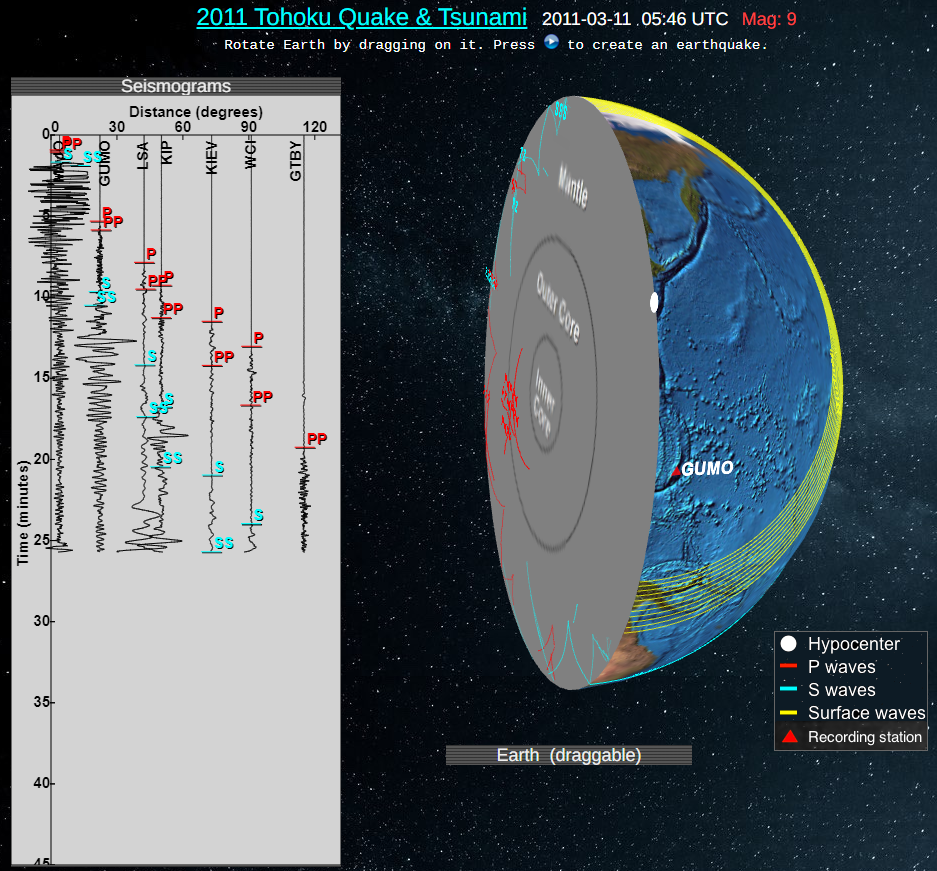
\includegraphics[scale=0.15]{iris}
	\end{wrapfigure}
	\begin{itemize}
	\item Beispiel für mechanische Wellen
	\item Erdbeben versetzt umgebende Teilchen in Bewegung
	\item Bewegung breitet sich über Globus aus
	\item unterschiedliche Arten von Bewegung
	\item Seismografen registrieren die Bewegung
	\end{itemize}
	\url{http://ds.iris.edu/seismon/swaves/}
}

\frame
{
  \frametitle{Ziele für die heutige Unterrichtseinheit}
  \textbf{Wie viel Zeit bleibt um sich vor den gefährlichen Oberflächenwellen eines Erdbebens in Sicherheit zu bringen?}
  \begin{itemize}
	\item Gemeinsamkeiten und Unterschiede von Schwingungen und Wellen
	\item Wellenarten
	\item Wellenlänge und Ausbreitungsgeschwindigkeit
	\item Experiment Ausbreitungsgeschwindigkeit
	\item Übungsaufgaben
	%\item Berechnung der Zeit zwischen den schnellen Transversal- und Longitudinal-wellen und den Oberflächenwellen bei einem Erdbeben.
  \end{itemize}
}

\frame
{
  \frametitle{Von der Schwingung zur Welle}
  \textbf{Gekoppelte Pendel}
	\begin{wrapfigure}{l}{4cm}
	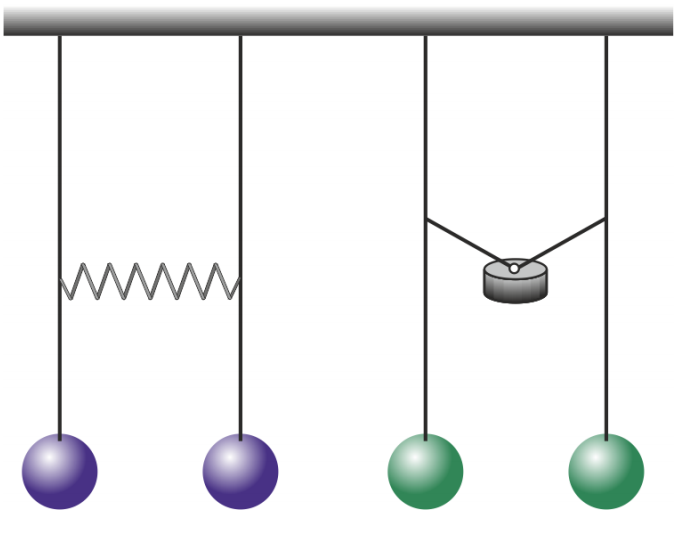
\includegraphics[scale=0.2]{Pendel_gekoppelt}
	\end{wrapfigure}
	\begin{itemize}
	\item einfachste Form der Ausbreitung
	\item Pendel sind \textbf{gekoppelt} (Feder oder Masse)
	\item 1. Pendel gibt seine Energie an 2. Pendel ab
	\item Und umgekehrt (2. Pendel $\rightarrow$ 1. Pendel)
	\item mathematisch dargestellt im Auslenkungs-Zeit-Diagramm
	\end{itemize}
	\url{https://www.walter-fendt.de/html5/phde/coupledpendula_de.htm}
}

\frame[allowframebreaks]
{
  \frametitle{Erweiterung auf mehrere Schwinger}
  \textbf{Wellenmaschine mehrere gekoppelte Elemente}
	%\begin{wrapfigure}{l}{4cm}
	%\animategraphics[loop, autoplay, width=4cm]{25}{Wavemachine-}{148}{0}
	%\end{wrapfigure}
	\begin{itemize}
	\item Kopplung mehrerer Schwinger
	\item Schwingung breitet sich im Raum aus
	\item Geschwindigkeit und Beschleunigung ändern sich zeitlich periodisch $\rightarrow$ Schwingung
	\item Zusätzlich \textbf{räumlich} periodische Änderung $\rightarrow$ Welle
	\item Energie wird übertragen, kein Stoff
	\end{itemize}
	\begin{block}{Definition}
	Eine mechanische Welle ist die Ausbreitung einer mechanischen Schwingung im Raum.
	\end{block}
	\begin{block}{Definition}
	Eine Welle ist eine zeitlich und räumlich periodische Änderung physikalischer Größen.
	\end{block}
	\begin{block}{Definition}
	Mit einer Welle wird Energie übertragen, jedoch kein Stoff transportiert.
	\end{block}
}

\frame[allowframebreaks]
{
  \frametitle{mathematische Beschreibung}
	\begin{block}{harmonische Schwingung}
	\begin{align*}
	y=y_{max}\cdot\sin \left( \dfrac{2\pi}{T}\cdot t\right) 
	\end{align*}
	$T\quad$Schwingungsdauer; $t\quad$Zeit
	\end{block}
	\begin{block}{harmonische Welle}
	\begin{align*}
	y=y_{max}\cdot\sin 2\pi\left( \dfrac{t}{T}-\dfrac{x}{\lambda}\right) 
	\end{align*}
	$T\quad$Schwingungsdauer; $t\quad$Zeit; $x\quad$ Ort; $\lambda\quad$ Wellenlänge
	\end{block}	
}

\frame
{
  \frametitle{Ausbreitung einer Wellen}
  Momentaufnahmen einer Welle zu unterschiedlichen Zeiten
  \begin{tikzpicture}
  	\foreach \y in {0, ..., 8} {
  	  \draw[scale=0.3, domain=0:5*pi, smooth, variable=\x, samples=50] plot ({\x}, {sin(deg(\x-2*\y*pi/8))-\y*2});
      \draw[->, >=latex] (0,-2*0.3*\y) node[left] {$y_{max}\cdot\sin 2\pi(\frac{\y}{8T}-\frac{x}{\lambda}); t=\frac{\y}{8T}$} -- (0.3*pi*5.5,-2*0.3*\y) node[below] {$x$};
      \draw[->, >=latex, red] (\y*pi/4*0.3+pi/2*0.3,2*0.3-2*\y*0.3) -- (\y*pi/4*0.3+pi/2*0.3,1*0.3-2*\y*0.3);
    }
    \draw[->, >=latex] (0,-0.3*17) -- (0,0.3*1.5) node [left] {$y$};
    %\draw (-15*0.3,pi/2) -- (-18*0.3,0);
    \draw[red, thin] (5*pi/4*0.6,1*0.3) -- (5*pi/4*0.6,2*0.3);
    %\draw[red, thin] (9*pi/4*0.6,1*0.3) -- (9*pi/4*0.6,2*0.3);
    \draw[<->, >=latex, red] (1*pi/4*0.6,0.5) -- node [above] {$\lambda$} (5*pi/4*0.6,0.5) ;
  \end{tikzpicture}
}

\frame[allowframebreaks]
{
  \frametitle{Physikalische Kenngrößen}
	\begin{block}{Wellenlänge}
	Die Wellenlänge ist der minimale Abstand zwischen zwei Oszillatoren, die sich im gleichen Schwingungszustand befinden. Das ist auch der Abstand zwischen zwei benachbarten Wellenbergen oder Wellentälern.\\
	Formelzeichen: $\lambda$\\
	Einheit: ein Meter (\SI{1}{\meter})
	\end{block}
}

\frame
{
  \frametitle{Eine Harmonische Welle}
  \begin{block}{y-x-Diagramm}
  \begin{tikzpicture}
	\draw[scale=0.3, domain=0:26/5*pi, smooth, blue, variable=\x, samples=50] plot ({\x}, {2*sin(deg(\x});
	\draw[->, >=latex] (0,0) node[left] {$ $} -- (0.3*pi*5.5,0) node[below] {$x$};
    \draw[->, >=latex] (0,-0.8) -- (0,1.1) node [left] {$y$};
    %\draw (-15*0.3,pi/2) -- (-18*0.3,0);
    \draw[blue, thin] (5*pi/4*0.6,2*0.3) -- (5*pi/4*0.6,1);
    \draw[blue, thin] (1*pi/4*0.6,2*0.3) -- (1*pi/4*0.6,1);
    \draw[<->, >=latex, blue] (1*pi/4*0.6,3*0.3) -- node [above] {$\lambda$} (5*pi/4*0.6,3*0.3) ;
  \end{tikzpicture}
  \end{block}
  \begin{block}{y-t-Diagramm}
  \begin{tikzpicture}
	\draw[scale=0.3, domain=0:26/5*pi, smooth, red, variable=\x, samples=50] plot ({\x}, {2*sin(deg(\x});
	\draw[->, >=latex] (0,0) node[left] {$ $} -- (0.3*pi*5.5,0) node[below] {$t$};
    \draw[->, >=latex] (0,-0.8) -- (0,1.1) node [left] {$y$};
    %\draw (-15*0.3,pi/2) -- (-18*0.3,0);
    \draw[red, thin] (5*pi/4*0.6,2*0.3) -- (5*pi/4*0.6,1);
    \draw[red, thin] (9*pi/4*0.6,2*0.3) -- (9*pi/4*0.6,1);
    \draw[<->, >=latex, red] (5*pi/4*0.6,3*0.3) -- node [above] {$T$} (9*pi/4*0.6,3*0.3) ;
  \end{tikzpicture}
  \end{block}
}

\frame[allowframebreaks]
{
	\begin{figure}
	\includegraphics[scale=0.3]{wellenmaschine.png}
	\caption{graphische Darstellung mittels Gnuplot}
	\end{figure}
  \frametitle{Graphische Darstellung der Wellenmaschine}
%\url{file:///C:/Users/Denise_Heiko/Documents/latex/Gnuplot/Wellenmaschine.gif} 
\href{Wellenmaschine.gif}{Animation starten}
}

\frame[allowframebreaks]
{
  \frametitle{Wellenarten}  
	\begin{block}{Längswellen (Longitudinalwellen)}
	\begin{itemize}
	\item Schwingungsrichtung und Ausbreitungsrichtung stimmen überein
	\item z.B.: Schallwellen in Luft oder Wasser, lange Spiralfeder
	\end{itemize}
	\end{block}
	\begin{figure}
	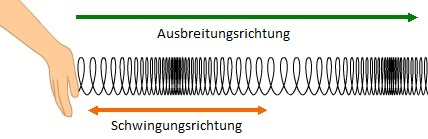
\includegraphics[scale=0.4]{längswelle.jpg}
	\caption{Demoexperiment Querwelle}
	\end{figure}

	\begin{block}{Querwellen (Transversalwellen)}
	\begin{itemize}
	\item Schwingungsrichtung und Ausbreitungsrichtung verlaufen senkrecht zueinander
	\item z.B.: Seilwellen, ein Teil der Erdbebenwellen
	\end{itemize}
	\end{block}
	\begin{figure}
	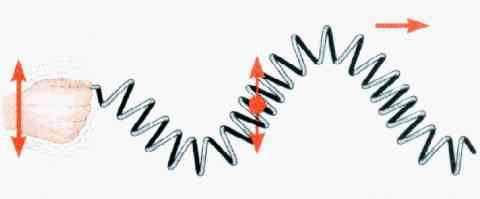
\includegraphics[scale=0.3]{Querwelle}
	\caption{Demoexperiment Querwelle}
	\end{figure}
	\begin{block}{Oberflächenwellen (Kreiswellen)}
	\begin{itemize}
	\item Teilchen führen kreisförmige Bewegung aus
	\item treten an Oberflächen auf
	\item z.B.: Wasserwellen
	\end{itemize}
	\end{block}
	\begin{figure}
		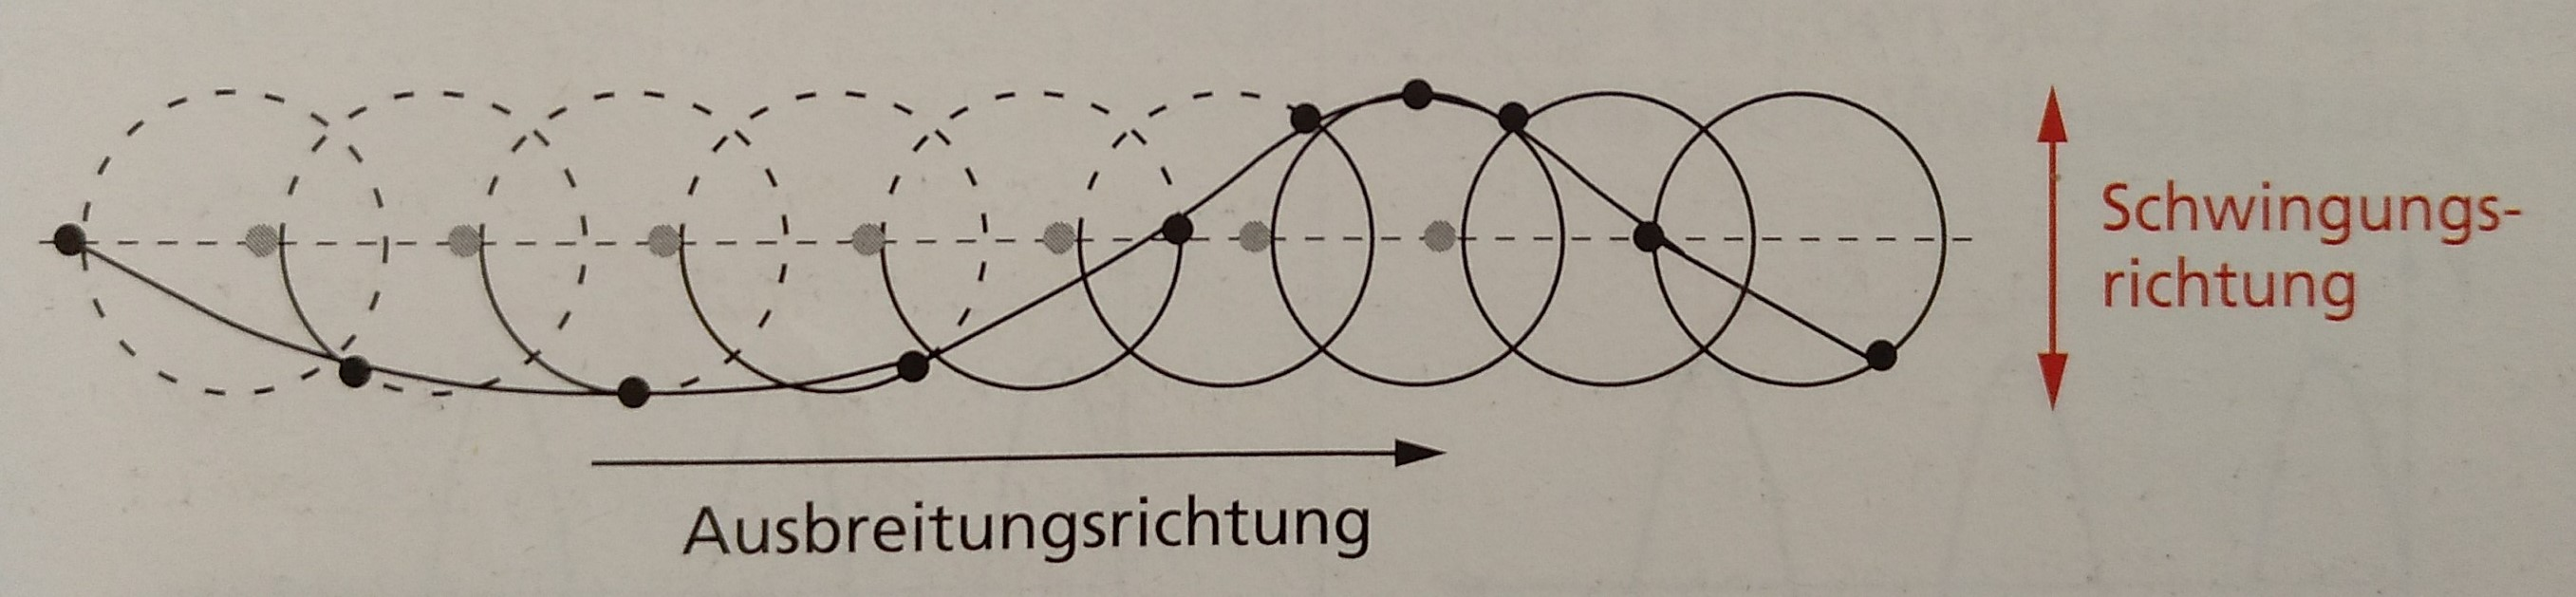
\includegraphics[scale=0.1]{kreiswellen.jpg}
		\caption{Darstellung von Kreiswellen}
	\end{figure}
	\href{wasser.gif}{Animation starten}
}

\frame
{
  \frametitle{Zusammenhang zwischen Ausbreitungsgeschwindigkeit und Wellenlänge}
	\begin{block}{Ausbreitungsgeschwindigkeit}
	Die Ausbreitungsgeschwindigkeit einer Welle ist die Geschwindigkeit, mit der sich eine bestimmte Phase im Raum ausbreitet.\\
	Formelzeichen: v\\
	Einheit: ein Meter durch Sekunde (\SI{1}{\meter\per\second})
	\end{block}
	\begin{block}{Ausbreitungsgeschwindigkeit}
	Für alle mechanischen Wellen gilt:\\
	$v=\lambda\cdot f\quad$ oder $\quad v=\frac{\lambda}{T}\quad$ mit $\quad f=\frac{1}{T}$\\
	Formelzeichen: v\\
	Einheit: ein Meter pro Sekunde (\SI{1}{\meter\per\second})
	\end{block}	
}

\frame
{
  \frametitle{Ausbreitungsgeschwindigkeit von Schallwellen}
	Mit zwei Smartphones kann die Schallgeschwindigkeit gemessen werden. Die App \textit{phyphox} auf den beiden Smartphones bestimmt dabei die Zeitspanne, die der Schall benötigt, um eine vorgegebene Strecke zu durchlaufen.\\
\url{https://www.youtube.com/watch?v=-XSTRqhJ6MQ}\\
$\rightarrow$ Durchführung des Versuches
}

\frame
{
\frametitle{Beispielaufgabe 1 Wellenlänge Schallwelle}
\textbf{Aufgabe:} Die vom menschlichen Ohr wahrnehmbaren Schallwellen haben eine Frequenz zwischen ca. \SI{20}{\hertz} und \SI{20000}{\hertz} und die Schallgeschwindigkeit beträgt ca. \SI{340}{\meter\per\second}.\\
\begin{enumerate}
	\item Berechnen Sie die Wellenlänge $\lambda$ einer Schallwelle bei $f=\SI{1000}{\hertz}$.
	\item Wie groß ist die Periodendauer in diesem Fall?
\end{enumerate}
}
\frame
{
\textbf{Lösung:}
\begin{enumerate}
\item 
	\begin{align*}
	v=\lambda\cdot f\Rightarrow\lambda=\dfrac{v}{f}=\dfrac{\SI{340}{\meter\per\second}}{\SI{1000}{\per\second}}=\SI{0,34}{\meter}
	\end{align*}
	\newpage
\item
	\begin{align*}
	T&=\dfrac{1}{f}=\dfrac{1}{\SI{1000}{\per\second}}=\SI{0,001}{\second}\quad\text{bzw.}\\
	v=\dfrac{\lambda}{T}\Rightarrow T&=\dfrac{\lambda}{v}=\dfrac{\SI{0,34}{\meter}}{\SI{340}{\meter\per\second}}=\SI{0,001}{\second}
	\end{align*}
\end{enumerate}
}

\frame
{
\frametitle{Beispielaufgabe 2 Wellenlänge Schallwelle}
\uncover<1->
{
\textbf{Aufgabe:} Welche Frequenz hat ein Erreger, der in Luft ($v=\SI{340}{\meter\per\second}$) eine Schallwelle mit der Wellenlänge \SI{20}{\centi\meter} erzeugt?\\
}
\uncover<2->
{
\textbf{Lösung:}
\begin{align*}
v=\lambda\cdot f\Rightarrow f=\dfrac{v}{\lambda}=\dfrac{\SI{340}{\meter\per\second}}{\SI{20}{\centi\meter}}=\dfrac{\SI{340}{\meter\per\second}}{\SI{0,20}{\meter}}=\SI{1700}{\per\second}
\end{align*}
}
}

\frame
{
\frametitle{Beispielaufgabe 3 Wellenlänge Schallwelle}
\uncover<1->
{
\textbf{Aufgabe:} Bei einer Echolotmessung sendet eine Schallquelle ($f=\SI{40000}{\hertz}$) unter Wasser Schallwellen mit der Wellenlänge $\lambda=\SI{3,7}{\centi\meter}$ aus. Wie groß ist die Ausbreitungsgeschwindigkeit des Schalls in Wasser?\\
}
\uncover<2->
{
\textbf{Lösung:}
\begin{align*}
v=\lambda\cdot f=\SI{3,7}{\centi\meter}\cdot\SI{40000}{\hertz}=\SI{0,037}{\meter}\cdot\SI{40000}{\per\second}=\SI{1480}{\meter\per\second}
\end{align*}
}
}

\frame
{
\frametitle{Beispielaufgabe 4 Erdbeben}
\uncover<1->
{
\textbf{Aufgabe:} Im Jahr 1985 ereignete sich in Mexiko ein schweres Erdbeben. Das Epizentrum lag \SI{340}{\kilo\meter} von Mexiko City entfernt. Zunächst trafen in der Hauptstadt die P-Wellen ein, die sich mit einer Geschwindigkeit von \SI{6}{\kilo\meter\per\second} ausbreiten. Berechnen Sie die Zeit, die den Bewohnern blieb, um sich vor den gefährlichen Oberflächenwellen ($v=\SI{3}{\kilo\meter\per\second}$) in Sicherheit zu bringen.\\
}

\uncover<2->
{
\textbf{Lösung:}
  \begin{tikzpicture}[scale = 0.07]
	\draw[smooth, red,] (0,0) -- node [above, rotate=17] {$v_O=\SI{3}{\kilo\meter\per\second}$} (112,34.0);
	\draw[smooth, blue,] (0,0) -- node [above, rotate=34] {$v_P=\SI{6}{\kilo\meter\per\second}$}(56,34.0);
	\draw[->, >=latex] (0,0) node [left] {Epizentrum} -- (120,0) node [below] {$t$};
    \draw[->, >=latex] (0,0) -- (0,38.0) node [left] {$s$};
    \draw[smooth, red, dotted, thin] (0,34) -- (112,34);
    \draw[smooth, blue, dotted, thin] (0,34) node [left] {Mexiko} -- (56,34);
    \draw[smooth, red, dotted, thin] (112,34) -- (112,-1) node [below] {$t_O$};
    \draw[smooth, blue, dotted, thin] (56,34) -- (56,-1) node [below] {$t_P$};
    \draw[<->, >=latex] (56,-10) -- node[above] {$\Delta t$} (112,-10);
    %\draw (-15*0.3,pi/2) -- (-18*0.3,0);
    %\draw[red, thin] (5*pi/4*0.6,2*0.3) -- (5*pi/4*0.6,1);
    %\draw[red, thin] (9*pi/4*0.6,2*0.3) -- (9*pi/4*0.6,1);
    %\draw[<->, >=latex, red] (5*pi/4*0.6,3*0.3) -- node [above] {$T$} (9*pi/4*0.6,3*0.3) ;
  \end{tikzpicture}
}
}

\frame
{
\textbf{Lösung:}
  \begin{tikzpicture}[scale = 0.07]
	\draw[smooth, red,] (0,0) -- node [above, rotate=17] {$v_O=\SI{3}{\kilo\meter\per\second}$} (112,34.0);
	\draw[smooth, blue,] (0,0) -- node [above, rotate=34] {$v_P=\SI{6}{\kilo\meter\per\second}$}(56,34.0);
	\draw[->, >=latex] (0,0) node [left] {Epizentrum} -- (120,0) node [below] {$t$};
    \draw[->, >=latex] (0,0) -- (0,38.0) node [left] {$s$};
    \draw[smooth, red, dotted, thin] (0,34) -- (112,34);
    \draw[smooth, blue, dotted, thin] (0,34) node [left] {Mexiko} -- (56,34);
    \draw[smooth, red, dotted, thin] (112,34) -- (112,-1) node [below] {$t_O$};
    \draw[smooth, blue, dotted, thin] (56,34) -- (56,-1) node [below] {$t_P$};
    \draw[<->, >=latex] (56,-10) -- node[above] {$\Delta t$} (112,-10);
    %\draw (-15*0.3,pi/2) -- (-18*0.3,0);
    %\draw[red, thin] (5*pi/4*0.6,2*0.3) -- (5*pi/4*0.6,1);
    %\draw[red, thin] (9*pi/4*0.6,2*0.3) -- (9*pi/4*0.6,1);
    %\draw[<->, >=latex, red] (5*pi/4*0.6,3*0.3) -- node [above] {$T$} (9*pi/4*0.6,3*0.3) ;
  \end{tikzpicture}
\begin{align*}
t=\dfrac{s}{v}\quad\Rightarrow \quad \Delta t&=t_O-t_P=\dfrac{s}{v_O}-\dfrac{s}{v_P}=\dfrac{\SI{340}{\kilo\meter}}{\SI{3}{\kilo\meter\per\second}}-\dfrac{\SI{340}{\kilo\meter}}{\SI{6}{\kilo\meter\per\second}}\\
&=\dfrac{170}{3}\si{\second}\approx\SI{56,7}{\second}
\end{align*}
}
\end{document}
